\section{Likelihood of long-run frequencies}\label{sec:likelihood} 

%Claudia Examples with equally likely long-run freqs – we can have very different
%longrun MI leading to same sample MI. Introduced by a discrete example.
%Multinomial probabilities

In the previous section we introduced the definition of Mutual Information between stimulus and responses (some measure/parametrization of neural activity), as a function of the long-run conditional frequencies of the responses on the stimulus. Unfortunately, for any biological neural system, the long-run frequencies are unknown, while what we have at our disposal is typically a limited\footnote{limited is a vague word. In this work we consider a sample limited if the number of datapoints is of the same order of magnitude of the possible combinations of stimulus and response value.} sample drawn from these unknown long-run frequencies. In order to compute the mutual information between stimulus and response, we hence want to use our data to make a guess of the long-run frequencies. How can we tell which long-run frequencies would most likely have generated our data? Let's think at the problem in reverse: if we knew the long-run frequencies then the likelihood $P(\hat{s}\vert \mathbf{f_s})$ would tell us how likely is our sample. It follows that for in the case of unknown long-run frequencies, the likelihood of \textit{candidate} long-run frequencies for our data can instruct us on how likely they might have generated the sample. How to choose the candidate long-run frequencies though? And, should be the likelihood the only metric for appraising long-run frequencies? One might be tempted to chose as a candidate only the long-run frequencies that maximize the likelihood for our data, namely the sample frequencies. Let's see why this problematic for a limited sample:

\begin{enumerate}
\item By choosing the maximum likelihood estimator of the long-run frequencies, one disregards completely other long-run frequencies which might have only a slightly smaller likelihood. Intuitively this is not a big issue, if the mutual info between stimulus and response for the disregarded long-run frequencies is similar to the mutual information associated to the maximum likelihood (sample) long-run frequencies. This might not always be the case, see the continuation of Example 1 in sec.~\ref{example1_con1}. 

\item By choosing the sample frequencies as the only candidate long-run frequencies for our data one approaches the sample in a completely agnostic fashion. This means that the assumption made by this choice is that the researcher doesn't have any kind of pre-sample knowledge about what the biologically plausible candidate long-run frequencies are, which is: every long-run frequency is attained as equally likely until the sample is collected. This is often not true for at least two reasons:
\begin{enumerate}

\item the exactly same neural system might have been probed before, providing us some evidence in favor of some candidate long-run frequencies;

\item biological constraints on the long-run frequencies for the system under investigation might be well established and be reported in the literature.

\end{enumerate}

\item By choosing the maximum-likelihood frequencies and computing the mutual information from them, one typically disregards the actual value of the likelihood. This value might be instead exploited to express our degree of belief (and uncertainty) on our mutual information estimate, as inherited from the degree of belief on the long-run frequencies that we chose (in this case the sample ones).

\item mutual info bias?

\end{enumerate}

In the next section we will see how a logical approach to the estimate of the long-run frequencies can address these issues regarding the mutual information.

\subsection{Example 1 continued. Mutual Infromation of high likelihood long-run frequencies.}\label{example1_con1}

Consider now the sample introduced in sec. \ref{example1}, for which we are aiming at an estimate of the mutual information between the spike count (r) of this neuron and the north/south head direction (s). The mutual information is a function of the long-run frequencies and the likelihood of long-run frequencies tells us how probably the sample was generated from them. Given the long-run frequencies $\mathbf{f_s}=\{f_s(r)\}_{s,r}$ their likelihood for our sample $\hat{s}$ is:

\begin{equation}
P(\hat{s}\vert \mathbf{f_s})=\prod_{s,r} f_s(r)^{N\hat{f}_s(r)}
%\frac{N!}{\prod_{s,r} \hat{f}_s(r)!}\prod_{s,r} f_s(r)^{N\hat{f}_s(r)}
\label{eq:categorical_likelihood}
\end{equation}

where $\hat{f}_s(r)$ are the sample frequencies shown in Fig.~\ref{fig:sample_frequencies}. The probability distribution in Eq. \eqref{eq:categorical_likelihood} is the categorical one and it assumes that the probability of response $r$ given that the stimulus is $s$ is  $f_s(r)$ at each time step independently.

In Fig.\ref{fig:highlike_long-run_freqs} three examples of long-run frequencies with high likelihood (log-likelihood within $10\%$ of maximum log-likelihood) for the sample $\hat{s}$ in sec. \ref{example1} are displayed. Although these long-run frequencies might have generated our data with similar probability (likelihood), they yield rather different values of mutual information between spike count and head direction ( MIs at least $50\%$ apart). Therefore the examples in Fig.\ref{fig:highlike_long-run_freqs} suggest that the sample mutual information (bottom of Fig.\ref{fig:highlike_long-run_freqs}) alone \-- for limited sample sizes \--   might be poorly representative of the spectra of mutual information values corresponding to high-likelihood long-run frequencies. So if a single estimator of the mutual information based on solely the likelihood of the long-run frequencies is not a good estimator of the mutual info: how to construct a better one?

\begin{figure}
\centering
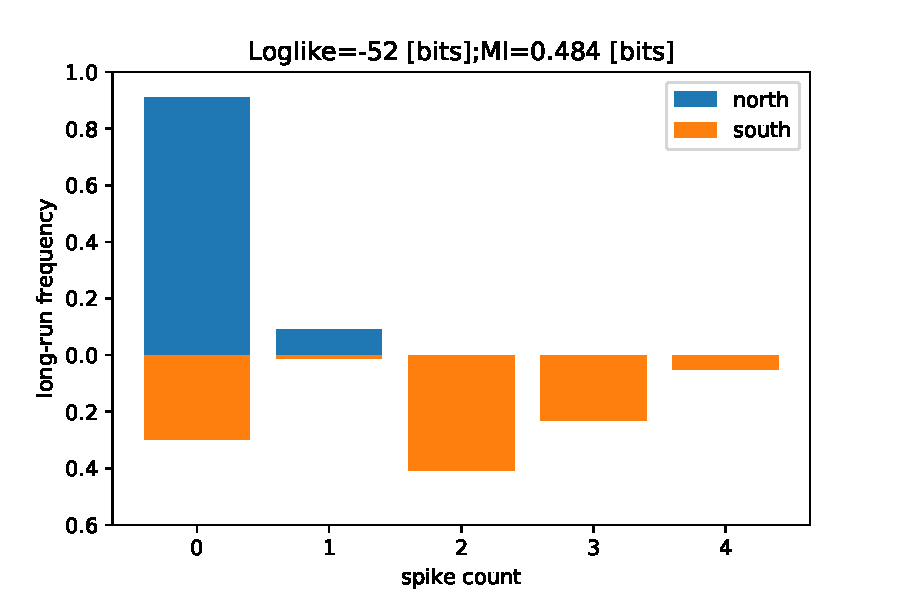
\includegraphics[scale=0.5]{HighLike_Plots0.pdf}\\
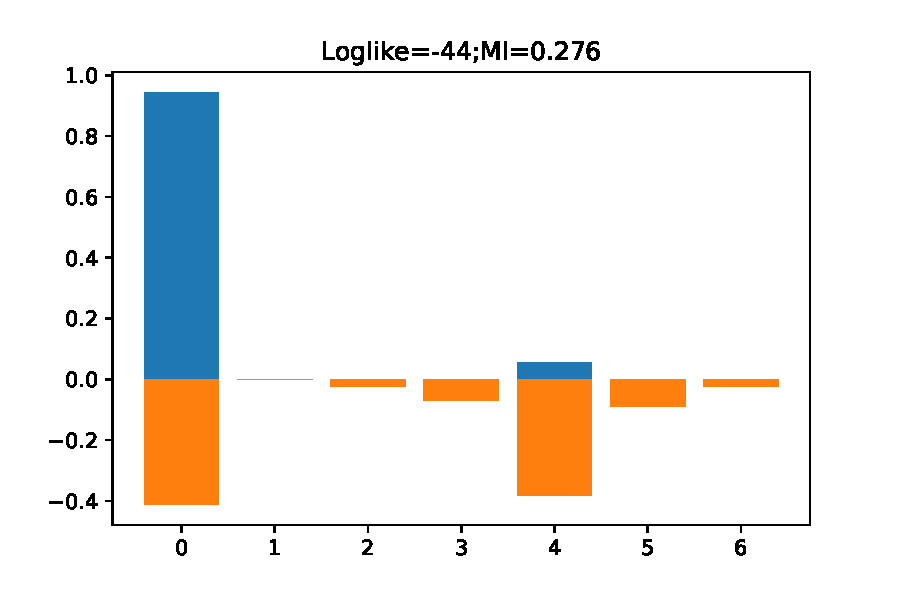
\includegraphics[scale=0.5]{HighLike_Plots1.pdf}\\ 
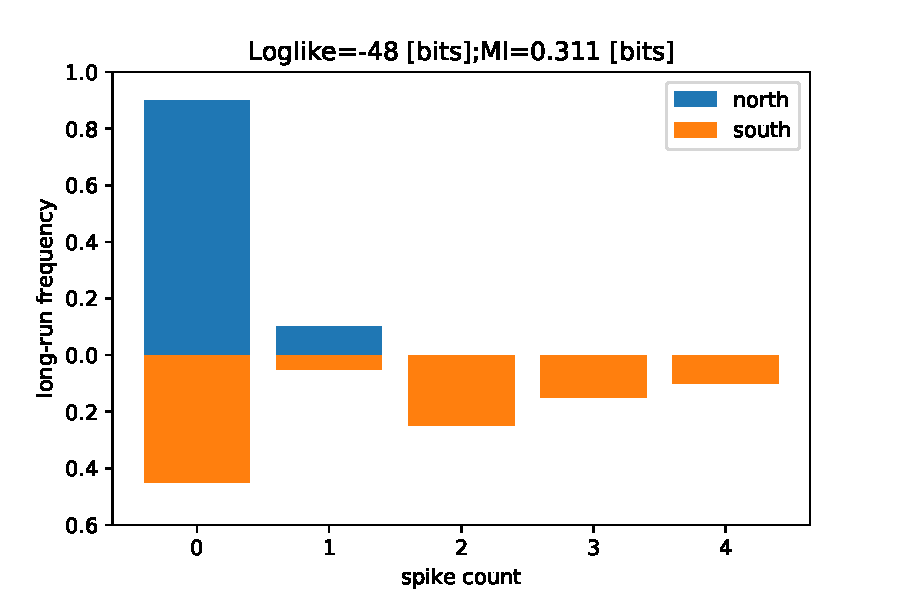
\includegraphics[scale=0.5]{HighLike_Plots_MaxLike.pdf} 
\label{fig:highlike_long-run_freqs}
\caption{High likelihood long-run frequencies for the data in sec. \ref{example1}. Examples of high likelihood long-run frequencies corresponding to high MI (top), low MI (center). Maximum likelihood long-run frequencies (bottom).}
\end{figure}

